

\chapter{排列、组合、二项式定理}


排列与组合的内容是学习二项式定理，概率的预备知识，也是进一步学习组合分析、系统控制、计算机理论等的必备基础。由于它的方法特殊，所以这部分知识在发展逻辑思维能力上有它独特的作用。

二项式定理揭示了二项式的正整数次幂的展开法则。它是在乘法公式及组合数公式的基础上学习的内容。它与概率论，微积分中的一些知识有密切的联系，是进一步学习数学时经常用到的基础知识。

\section*{一、排列与组合}

\section{基本原理}

先看下面的具体问题。

从甲地到乙地，可以乘火车，也可以乘汽车，还可以乘轮船。一天中，火车有4班，汽车有2班，轮船有3班。那么一天中乘坐这些交通工具从甲地到乙地共有多少种不同的走法？

因为一天中乘火车有4种走法，乘汽车有2种走法，乘轮船有3种走法，每一种走法都可以从甲地到达乙地，因此，一天中乘坐这些交通工具从甲地到乙地共有
$$4+2+3=9$$种不同的走法。

在这个问题中，首先要弄清楚要完成的事是“一天中乘交通工具从甲地到达乙地”。第二，要清楚完成它有几类办法（在这里是有3种走法：乘火车，乘汽车，乘轮船）。第三，要清楚各类办法中分别有几种不同的方法，在这个问题里，第一类办法（乘火车）有4种不同的方法（火车有4班，每一班都是一种方法）；第二类办法（乘汽车）有2种不同的方法（汽车有2班，每班都是一种方法）；第三类办法（乘轮船）有3种不同的方法（轮船有3班，每班都是一种方法），所以完成“一天中乘交通工具从甲地到乙地”这件事共有$4+2+3  =9$种不同的方法。

一般地，解决这类问题用下面的原理：

\begin{thm}
{加法原理} 做一件事，完成它有$n$类办法，在第一类办法中有$m_{1}$ 种不同的方法，在第二类办法中有$m_{2}$ 种不同的方法，……，在第$n$类办法中有$m_{n}$种不同的方法。那么完成这件事共有    
\[N=m_{1}+m_{2}+\cdots +m_{n}\]
种不同的方法。
\end{thm}

\begin{remark}
“做一件事，完成它可以有$n$类办法”。这里是对完成这件事的\textbf{所有}方法的一个\textbf{分类}。分类时，首先要根据问题的特点确定一个分类的标准，标准不同，分类的结果也就不同。其次，分类应满足一个基本的要求：完成这件事的任何一种方法必属于某一类，并且分别属于不同两类的两种方法都是不同的方法。即各类办法中的方法组成的每个集合彼此的交集必须是空集，而它们的并集是全集。只有满足这样的分类时，才能使用加法原理。    
\end{remark}

\begin{example}
    找1—10中的所有合数，用如下方法：

第一类办法是找含有因数2的合数，有4、6、8、10四个合数；

第二类办法是找含有因数3的合数，有6、9二个合数；

第三类办法是找含有因数5的合数，有10一个合数。

则$N=4+2+1=7$个合数。
\end{example}

而实际上共有$4$、$6$、$8$、$9$、$10$五个合数。问题出在哪里呢？

显然，在上述的例子中，由于没有正确使用分类标准，故导致错误的结论。

我们再看另一类问题，具体例子如下：

由$A$村去$B$村的道路有3条，由$B$村去$C$村的道路有2条（图7.1）。从$A$村经过$B$村去$C$村，共有多少种不同的走法？

\begin{figure}[htp]
    \centering
\begin{tikzpicture}[>=stealth]
\node (A) at (0,0){$A$村};
\node (B) at (4,0){$B$村};
\node (C) at (8,0){$C$村};
\draw[->](A) --node[above]{中} (B) ;
\draw[->](A) to [bend left=35]node[above]{北} (B) ;
\draw[->](A) to [bend left=-35]node[below]{南} (B) ;
\draw[->](B)  to [bend left=30]node[above]{北}  (C) ;
\draw[->](B)  to [bend left=-30]node[below]{南}  (C) ;



\end{tikzpicture}
    \caption{}
\end{figure}

这里，从$A$村到$B$村有3种不同的走法，按这3种走法中
的每一种走法到达$B$村后，再从$B$村到$C$村又有2种不同的走法，因此，从$A$村经$B$村去$C$村共有
\[3\x 2=6\]
种不同的走法。

根据题意，这里要完成的事是“由$A$村经$B$村到$C$村”。要
完成这件事要分成两个步骤。第一步：“由$A$村到$B$村”。第二步：“由$B$村到$C$村”。又知道，完成第一步的方法有3种（有 3条路由$A$村通向$B$村），完成第二步的方法有2种（有2条路由$B$村通向$C$村）。当这两步都完成后才算完成了“由$A$村经$B$村到$C$村”这件事，所以完成的方法是$3\x  2=6$种。

一般地，对这一类问题我们有下面的原理。
\begin{thm}
    {乘法原理} 做一件事，完成它需要分成$n$个步骤，做第一步有$m_{1}$ 种不同的方法，做第二步有$m_{2}$ 种不同的方法，……，做第$n$步有$m_{n}$ 种不同的方法。那么完成这件事共有
\[
N=m_{1}\x m_{2}\x\cdots \x m_{n}
\]
种不同的方法。
\end{thm}


乘法原理和加法原理有哪些区别呢？

它们应用的对象在“完成一件事”的方式上是不同的：加法原理适用的问题中，“完成一件事”可以有不同类的办法，每一类办法中又有不同的方法，而每种方法，只需使用一次，即可“完成这件事”；而乘法原理所适用的问题中，“完成一件事”必须分成几个步骤，每个步骤中又有各种方法，用任何一种方法都不能“完成”这件事，这里的每一种方法只是完成几个步骤中的某一步。而只有依次将各个步骤都完成以后，这件事才能完成。

我们看下面这些实例，注意对所选用原理的理由的分析。

\begin{example}
    书架上层放有6本不同的数学书，下层放有5本不同的语文书。
\begin{enumerate}[(1)]
    \item 从中任取一本，有多少种不同的取法？
    \item 从中任取数学书与语文书各一本，有多少种不同的取法？
\end{enumerate}
\end{example}

\begin{analyze}
\begin{enumerate}[(1)]
    \item 这里“从中取出一本”是“一件事”，无论从书架的上层或下层去取，只要取出一本，这件事就完成了，完成这件事不须分步，任何一种取法只需用一次，即可完成，所以应该用加法原理。
    \item 这里“一件事”是指“从中任取数学书与语文书各一本”。所以完成这件事需分步骤。第一步：取一本数学书，第二步：取一本语文书。只有两步都完成后，才算做完了这件事，所以应该用乘法原理。
\end{enumerate}
\end{analyze}

\begin{solution}
\begin{enumerate}[(1)]
    \item 从书架上任取一本书，有两类办法：第一类办法是从上层取数学书，可以从6本书中任取一本，有6种方法；第二类办法是从下层取语文书，可以从5本书中任取一本，有5种方法。根据加法原理，得到不同的取法的种数是
\[N=m_{1}+m_{2}=6+5=11\]
从书架上任取一本书，有11种不同的取法。
\item 从书架上任取数学书与语文书各一本，可以分成两个步骤完成：第一步取一本数学书，有6种方法；第二步取一本语文书，有5种方法。根据乘法原理，得到不同的取法的种数是
\[N=m_{1}\x m_{2}=6\x 5=30\]
从书架上取数学书和语文书各一本，有30种不同的方法。
\end{enumerate}
\end{solution}


\begin{example}
    将3封信投入5个信箱内，有多少种不同的投信方法？
\end{example}

\begin{analyze}
    本题的“做一件事”是指把三封信都投到信箱内。
因此需分三个步骤：第一步先投第一封信；第二步投第二封信；第三步投第三封信。这三个步骤都完成，才算做完这件事，因此，需用乘法原理来解决此题。
\end{analyze}

\begin{solution}
第一步先投第一封信，因为有5个信箱，所以有5种不同的投法；第二步投第二封信，同样有5种投法；第三步投第三封信，同样也有5种投法，这样根据乘法原理，共有不同的投法有
\[
N=5\x 5\x 5=5^{3}=125.\]

答：共有125种不同的投法。
\end{solution}

\begin{rmk}
    弄清问题中“完成一件事”的含义，是选用加法原理或乘法原理的关键。
\end{rmk}

这类问题是排列组合中所研究的一种典型问题。为能正确地掌握这种问题的解法，我们构造一个数学模型，来剖析这一类问题。看下面的例子。


\begin{example}
已知两个集合$A=\{a,b,c\}$, $ B=\{m,n,p,q,  r\}$。从$A$到$B$建立映射$f$。问可建立多少个不同的映射$f$?    
\end{example}

\begin{analyze}
首先应明确本题中的“这件事”是指做映射。而由映射的定义知道，建立映射这件事具体的就是给集合$A$中的每一个元素在$B$集合中找一个象。把这件事的内容分析清楚后，就很容易得到其解决的方法，即分成三个步骤分别给$A$集合的元素$a$、$b$、$c$在$B$集合中找象，当三个步骤全进行完，则一个映射就被建立了。因此可以使用乘法原理去解决。
\end{analyze}

\begin{solution}
    第一步，先给元素$a$在$B$中找象，因为$B$中共有5个元素，所以共有5种方法；第二步，给元素$b$在$B$中找象，同样有5种方法；第三步，给元素$c$在$B$中找象，同样也有5种方法。这样根据乘法原理，共可建立不同的映射数目为
\[N=5\x 5\x 5=5^{3}=125.\]

答：共可建立125个不同的映射。
\end{solution}

由例7.4可看出，它实际上是例7.3问题的数学模式。$A$集合中三个元素相当于例7.3中的三封信，$B$集合中的五个元素相当于例7.3中的五个信箱，所谓投信这件事，就是从$A$到$B$建立映射，有多少种不同的映射，就对应着有多少种不同的投信方法。

因此，这类问题都涉及到两个集合$A$和$B$，在它们之间建立映射。注意，这里的问题是从$A$到$B$建立映射，而不是从$B$到$A$建立映射。从映射的定义可知这两个映射是有区别的。在建立映射过程中，$A$集合中的元素不能重复使用，就是说在给$A$集合元素找象的过程中，不能同时给一个元素找两个或两个以上的象；而$B$集合中的元素可重复使用，就是说$B$集合中的元素可以同时为$A$中不同元素的象。根据映射的要求区分出两个集合后，就可选定集合$A$、$B$。这样再使用乘法原理解决这类问题时，就不会出错。

\section*{习题一}

\begin{enumerate}
  \item 一件工作可以用两种方法完成，有5人会用第一种方法，另有4人会用第二种方法，选出一个人来完成这件工作，共有多少种选法？
\item 在读书活动中，一个学生要从2本科技书、2本政治书、 3本文艺书里任选一本，共有多少种不同的选法？
    \item 从5本科技书、4本文艺书和3本政治书里各选出一本，共有多少种不同选法？
\item 乘积 $\left(a_{1}+a_{2}+a_{3}+a_{4}\right)\left(b_{1}+b_{2}+b_{3}\right)\left(c_{1}+c_{2}+c_{3}+c_{4}+c_{5}\right)$
  展开后共有多少项？  
  \item 如图，从甲地到乙地有2条路可通，从乙地到丙地有三条路可通；从甲地到丁地有4条路可通，从丁地到丙地有2条路可通。从甲地到丙地共有多少种不同的走法？
\begin{center}
\begin{tikzpicture}[>=stealth, scale=1.2]
\begin{scope}
\node[draw, circle](A) at (0,2){甲地};
\node[draw, circle](B) at (3,2){乙地};
\node[draw, circle](C) at (0,0){丁地};
\node[draw, circle](D) at (3,0){丙地};
\draw[->](A) to [bend left=15](B);
\draw[->](A) to [bend left=-15](B);
\draw[->](A) to [bend left=15](C);
\draw[->](A) to [bend left=-15](C);
\draw[->](A) to (C);
\draw[->](C) to [bend left=15](D);
\draw[->](C) to [bend left=-15](D);
\draw[->](B) to [bend left=15](D);
\draw[->](B) to [bend left=-15](D);
\draw[->](B) to (D);
\node at (1.5,-1){（第5题）};
\end{scope}
\begin{scope}[xshift=4.5cm]
\node(A) at (0,1.5){甲地};
\node(B) at (3.2,1.5){丙地};
\node(C) at (1.6,0){乙地};
\draw (A) to [bend left=30] (B);
\draw (A) to [bend left=15] (B);
\draw (A) to [bend left=15] (C);
\draw (A) to [bend left=-15] (C);
\draw (C) to [bend left=15] (B);
\draw (C) to [bend left=-15] (B);
\draw(C)--(B);

\node at (1.5,-1){（第6题）};
\end{scope}
\end{tikzpicture}
\end{center}  

    \item 如图，从甲地到乙地有2条路可走，从乙地到丙地有3条路可走，又从甲地不经过乙地到丙地有2条水路可走。
\begin{enumerate}[(1)]
    \item 从甲地经乙地到丙地有多少种不同的走法？
    \item 从甲地到丙地共有多少种不同的走法？
\end{enumerate}
    \item 一个口袋内装有5个小球，另一个口袋内装有4个小球，所有这些小球的颜色互不相同。
\begin{enumerate}[(1)]
    \item 从两个口袋内任取一球，有多少种不同的取法？
    \item 从两个口袋内各取一球，有多少种不同的取法？
\end{enumerate}

\item 已知$x\in\{1,2,3\}$, $y\in\{1,2,3,4,5\}$，问：可以组成多少个不同的点$P(x,y)$?

\item 由数字$0,1,2,3,4$可以组成多少个三位数（各位上的数字可以相同）？其中有多少个偶数？
\end{enumerate}
    

\section{排列}

先看两个具体问题。
\begin{thm}{问题1}
     北京、上海、广州三个民航站之间的直达航线，需要准备多少种不同的飞机票？
\end{thm}

要完成“准备飞机票”这件事，只需根据题意确定好“起点站”和“终点站”，即要完成这件事，须分两个步骤：第一步，确定“起点站”；第二步，确定“终点站”。按题意，“起点站”有3种确定方法；第二步，当选定起点站以后再来确定终点站，按题意，终点站只能在除去起点站以后的两个站中选，因此有2种方法。所以，根据乘法原理，需要准备的飞机票共有
\[3\x 2=6 \; \text{（种）}\]
也就是说，需要准备如下6种不同的飞机票：
\begin{center}
\begin{tikzpicture}[yscale=.8]
\node at (0,4){起点站};
\node at (3,4){终点站};	
\node at (6,4){飞机票};
\node (A)at (0,2.5){北京};	\node(A1) at (3,3){上海};	\node at (6,3){北京——上海};
\node(A2) at (3,2){广州};	\node at (6,2){北京——广州};
\node (B)at (0,.5){上海};	\node(B1) at (3,1){北京};	\node at (6,1){上海——北京};
\node(B2) at (3,0){广州};	\node at (6,0){上海——广州};
\node (C)at (0,-1.5){广州};	\node(C1) at (3,-1){北京};	\node at (6,-1){广州——北京};
\node(C2) at (3,-2){上海};	\node at (6,-2){广州——上海};

\draw(A)--(A1)  (A)--(A2);
\draw(B)--(B1)  (B)--(B2);
\draw(C)--(C1)  (C)--(C2);

\end{tikzpicture}
\end{center}


\begin{thm}
{问题2} 由数字$1,2,3,4$可以组成多少个没有重复数字的三位数？
\end{thm}

这个问题就是从$1,2,3,4$这四个数字中，每次取出三
个，按照百位、十位、个位的顺序排列起来，求一共有多少种不同的排法。

这个问题中，“完成一件事”就是“由数字$1,2,3,4$中选出三个，组成没有重复的三位数”，这可以分三步进行：

第一步，先排百位上的数字，在$1,2,3,4$这四个数字中任取一个，有4种方法；

第二步，排十位上的数字，当百位上的数字确定以后，十位上的数字只能从余下的三个数字中去取，有3种方法；

第三步，排个位上的数字，当百位、十位上的数字都确定以后，个位上的数字只能从余下的两个数字中去取，有2方法。

根据乘法原理，从四个不同的数字中，每次取出三个排成一个三位数的方法共有
\[4\x 3\x 2=24\;\text{（种）}\]
也就是说，可以排成24个不同的三位数。具体排法如下：

\begin{center}
\begin{tikzpicture}[decoration={text effects along path,
text effects/.cd,
path from text,
every letter/.style={shape=rectangle, draw}}]
\begin{scope}
\path [decorate, decoration={text={123}}] (4,3);
\path [decorate, decoration={text={124}}] (4,2);
\path [decorate, decoration={text={132}}] (4,1);
\path [decorate, decoration={text={134}}] (4,0);
\path [decorate, decoration={text={142}}] (4,-1);
\path [decorate, decoration={text={143}}] (4,-2);

\path [decorate, decoration={text={12?}}] (2,2.5);
\path [decorate, decoration={text={13?}}] (2,0.5);
\path [decorate, decoration={text={14?}}] (2,-1.5);
\path [decorate, decoration={text={1??}}] (0,0.5);

\draw[decorate, decoration={brace, mirror, amplitude=10pt}](1.75,2.5)--(1.75,-1.5);
\draw[decorate, decoration={brace, mirror, amplitude=5pt}](3.75,3)--(3.75,2);
\draw[decorate, decoration={brace, mirror, amplitude=5pt}](3.75,1)--(3.75,0);
\draw[decorate, decoration={brace, mirror, amplitude=5pt}](3.75,-1)--(3.75,-2);
\end{scope}
\begin{scope}[xshift=6.5cm]
\path [decorate, decoration={text={213}}] (4,3);
\path [decorate, decoration={text={214}}] (4,2);
\path [decorate, decoration={text={231}}] (4,1);
\path [decorate, decoration={text={234}}] (4,0);
\path [decorate, decoration={text={241}}] (4,-1);
\path [decorate, decoration={text={243}}] (4,-2);

\path [decorate, decoration={text={21?}}] (2,2.5);
\path [decorate, decoration={text={23?}}] (2,0.5);
\path [decorate, decoration={text={24?}}] (2,-1.5);
\path [decorate, decoration={text={2??}}] (0,0.5);

\draw[decorate, decoration={brace, mirror, amplitude=10pt}](1.75,2.5)--(1.75,-1.5);
\draw[decorate, decoration={brace, mirror, amplitude=5pt}](3.75,3)--(3.75,2);
\draw[decorate, decoration={brace, mirror, amplitude=5pt}](3.75,1)--(3.75,0);
\draw[decorate, decoration={brace, mirror, amplitude=5pt}](3.75,-1)--(3.75,-2);
\end{scope}
\end{tikzpicture}
\end{center}

\begin{center}
\begin{tikzpicture}[decoration={text effects along path,
text effects/.cd,
path from text,
every letter/.style={shape=rectangle, draw}}]
\begin{scope}
\path [decorate, decoration={text={312}}] (4,3);
\path [decorate, decoration={text={314}}] (4,2);
\path [decorate, decoration={text={321}}] (4,1);
\path [decorate, decoration={text={324}}] (4,0);
\path [decorate, decoration={text={341}}] (4,-1);
\path [decorate, decoration={text={342}}] (4,-2);

\path [decorate, decoration={text={31?}}] (2,2.5);
\path [decorate, decoration={text={32?}}] (2,0.5);
\path [decorate, decoration={text={34?}}] (2,-1.5);
\path [decorate, decoration={text={3??}}] (0,0.5);

\draw[decorate, decoration={brace, mirror, amplitude=10pt}](1.75,2.5)--(1.75,-1.5);
\draw[decorate, decoration={brace, mirror, amplitude=5pt}](3.75,3)--(3.75,2);
\draw[decorate, decoration={brace, mirror, amplitude=5pt}](3.75,1)--(3.75,0);
\draw[decorate, decoration={brace, mirror, amplitude=5pt}](3.75,-1)--(3.75,-2);
\end{scope}
\begin{scope}[xshift=6.5cm]
\path [decorate, decoration={text={412}}] (4,3);
\path [decorate, decoration={text={413}}] (4,2);
\path [decorate, decoration={text={421}}] (4,1);
\path [decorate, decoration={text={423}}] (4,0);
\path [decorate, decoration={text={431}}] (4,-1);
\path [decorate, decoration={text={432}}] (4,-2);

\path [decorate, decoration={text={41?}}] (2,2.5);
\path [decorate, decoration={text={42?}}] (2,0.5);
\path [decorate, decoration={text={43?}}] (2,-1.5);
\path [decorate, decoration={text={4??}}] (0,0.5);

\draw[decorate, decoration={brace, mirror, amplitude=10pt}](1.75,2.5)--(1.75,-1.5);
\draw[decorate, decoration={brace, mirror, amplitude=5pt}](3.75,3)--(3.75,2);
\draw[decorate, decoration={brace, mirror, amplitude=5pt}](3.75,1)--(3.75,0);
\draw[decorate, decoration={brace, mirror, amplitude=5pt}](3.75,-1)--(3.75,-2);
\end{scope}
\end{tikzpicture}
\end{center}


我们再分析一下上述两个问题的实质。第一个问题，是从3个不同的民航站中，每次取2个，然后按一定的顺序排成一列，求共有多少种不同的排法。第二个问题，就是从4个不同的数中，任取3个，然后排成一列，求共有多少种不同的排法。

再把上述问题抽象一下，把其中的民航站、数字叫做元素。那么上述两个问题可分别叙述如下：

问题1，就是从3个不同的元素中，任取2个，然后按一定的顺序排成一列，求一共有多少种不同的排法；问题2，就是从4个不同的元素中，任取3个，然后按一定的顺序排成一列，求一共有多少种不同的排法。

一般地说，从$n$个不同元素中，任取 $m\; (m\le  n)$ 个元素（本章只研究被取出的元素各不相同的情况），按照一定的顺序排成一列，叫做从$n$个不同元素中取出$m$个元素的一个排列。

\begin{remark}
    在排列定义中，提出“按照一定的顺序”，这里的“顺序”一词的含义是什么呢？

显然，这里的“顺序”一词并不是光指排队，实际上，“顺序”的含义是一个集合到另一个集合的单射。只要这两个集合之间构成一个集合到另一个集合的单射，我们就称之有“顺序”。如问题1中，起点站，终点站构成集合$A$，而北京、上海、广州三个民航站构成了集合$B$，如果$A$到$B$构成一个单射，即起、终点站分别对应B中的两个民航站，于是就构成了一种“顺序”。又如问题2中，个位，十位，百位构成集合$A$，而数字$1,2,3,4$构成集合$B$，于是排成某一三位数的问题转化成从$A$到$B$建立一种单射。由此可见，“按一定顺序排成一列”实质是建立两个集合之间的一种单射。

这样，排列我们也可如下定义：

集合$A$含有$m$个元素，集合$B$含有$n\; (n\ge m)$ 个元素，从集合A到集合B建立一种单射，叫做从$n$个不同元素中取出$m$个元素的一个排列。
\end{remark}


从排列的定义知道，如果两个排列相同，不仅这两个排列的元素必须相同，而且排列的顺序也必须完全相同。如果所取的元素不完全相同，例如问1中的飞机票“上海—北京”和“上海—广州”，它们就是两个不同的排列。即使所取的元素相同，但排列顺序不同，也不是相同的排列。如问题1中的飞机票“上海—北京”和“北京—上海”，虽然它们的元素相同，但排列顺序不同，也是两个不同的排列。

在实际问题中，有时需要写出某个排列问题的所有排列。为使所写出的排列既不重复，又不遗漏，需按一定的步骤才能完成这一工作。

例如，已知$a$、$b$、$c$、$d$这4个元素，写出每次取出3个元素的所有排列。我们可以这样来写：先考虑第一个位置上的元素，我们可以把$a$、$b$、$c$、$d$中任意一个元素写在第一个位置上，有4种写法；第一个位置上的元素写好后，第二个位置上的元素的写法就只有3种。如第一个位置上写了元素$b$，那么第二个位置上就只能写$a$、$c$、$d$三个元素。而当第二个位置上的元素写好后，第三个位置上的元素的写法就只有 2种。如第一、二个位置上分别写上元素$b$、$a$以后，第三个位置上就只能写$c$、$d$这两个元素。

从图7.2中可以清楚地看出，从4个元素$a$、$b$、$c$、$d$中每次取出3个元素所有的排列是：
\begin{figure}[htp]
    \centering
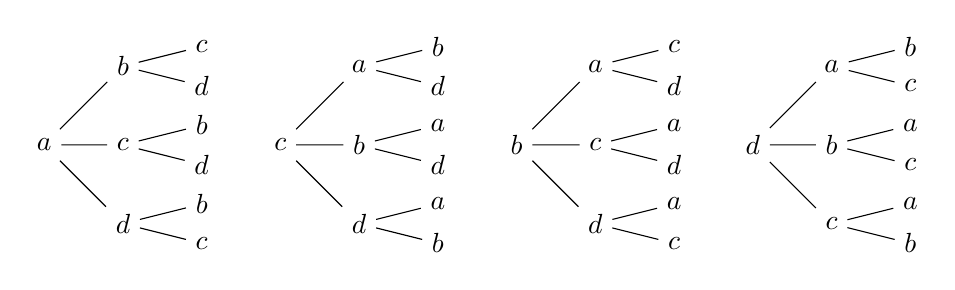
\begin{tikzpicture}[scale=.5]
\begin{scope}
    \node(A) at (0,0){$a$};
    \node(B1) at (2,2){$b$};
    \node(B2) at (2,0){$c$};
    \node(B3) at (2,-2){$d$};
    \node(C1) at (4,2.5){$c$};
    \node(C2) at (4,1.5){$d$};
    \node(C3) at (4,.5){$b$};
    \node(C4) at (4,-.5){$d$};
    \node(C5) at (4,-1.5){$b$};
    \node(C6) at (4,-2.5){$c$};
    \draw(A)--(B1) (A)--(B2) (A)--(B3);
    \draw(B1)--(C1) (B1)--(C2) (B2)--(C3) (B2)--(C4)  (B3)--(C5) (B3)--(C6) ;
\end{scope} 
\begin{scope}[xshift=6cm]
        \node(A) at (0,0){$c$};
    \node(B1) at (2,2){$a$};
    \node(B2) at (2,0){$b$};
    \node(B3) at (2,-2){$d$};
    \node(C1) at (4,2.5){$b$};
    \node(C2) at (4,1.5){$d$};
    \node(C3) at (4,.5){$a$};
    \node(C4) at (4,-.5){$d$};
    \node(C5) at (4,-1.5){$a$};
    \node(C6) at (4,-2.5){$b$};
    \draw(A)--(B1) (A)--(B2) (A)--(B3);
    \draw(B1)--(C1) (B1)--(C2) (B2)--(C3) (B2)--(C4)  (B3)--(C5) (B3)--(C6) ;
\end{scope} 
\begin{scope}[xshift=12cm]
         \node(A) at (0,0){$b$};
    \node(B1) at (2,2){$a$};
    \node(B2) at (2,0){$c$};
    \node(B3) at (2,-2){$d$};
    \node(C1) at (4,2.5){$c$};
    \node(C2) at (4,1.5){$d$};
    \node(C3) at (4,.5){$a$};
    \node(C4) at (4,-.5){$d$};
    \node(C5) at (4,-1.5){$a$};
    \node(C6) at (4,-2.5){$c$};
    \draw(A)--(B1) (A)--(B2) (A)--(B3);
    \draw(B1)--(C1) (B1)--(C2) (B2)--(C3) (B2)--(C4)  (B3)--(C5) (B3)--(C6) ;   
\end{scope} 
\begin{scope}[xshift=18cm]
         \node(A) at (0,0){$d$};
    \node(B1) at (2,2){$a$};
    \node(B2) at (2,0){$b$};
    \node(B3) at (2,-2){$c$};
    \node(C1) at (4,2.5){$b$};
    \node(C2) at (4,1.5){$c$};
    \node(C3) at (4,.5){$a$};
    \node(C4) at (4,-.5){$c$};
    \node(C5) at (4,-1.5){$a$};
    \node(C6) at (4,-2.5){$b$};
    \draw(A)--(B1) (A)--(B2) (A)--(B3);
    \draw(B1)--(C1) (B1)--(C2) (B2)--(C3) (B2)--(C4)  (B3)--(C5) (B3)--(C6) ;   
\end{scope}     
\end{tikzpicture}
    \caption{}
\end{figure}


\begin{center}
\begin{tabular}{cccccc}
$abc$  &   $abd$  &   $acb$  &   $acd$  &   $adb$  &   $adc$\\
$bac$  &   $bad$  &   $bca$  &   $bcd$  &   $bda$  &   $bdc$\\
$cab$  &   $cad$  &   $cba$  &   $cbd$  &   $cda$  &   $cdb$\\
$dac$  &   $dab$  &   $dba$  &   $dbc$  &   $dca$  &   $dcb$\\
\end{tabular}
\end{center}


\section{排列数公式}

从$n$个不同元素中取出$m\; (m\le  n)$ 个元素的所有排列的个数，叫做从$n$个不同元素中取出$m$个元素的排列数，用符号${\rm P}_{n}^{m}$表示\footnote{P是英文Permutation（排列）的第一个字母。}。

例如，从5个不同元素中取出2个元素的排列数记为${\rm P}_{5}^{2}$; 从4个不同元素中取出3个元素的排列数记为${\rm P}_{4}^{3}$.

现在我们研究计算排列数${\rm P}_{n}^{m}$的公式。先考虑$m=2$ 的情况。

求排列数$\perm{n}{2}$, 由排列数的定义就是求从$n$个不同的元素中取出2个元素的
所有排列的个数，假定有排好顺序的2个空位置（图7.3），从$n$个不同元素$a_{1},a_{2},\ldots,a_{n}$ 中任意取2个去填空，一个空位置填一个元素，每一种填法就得到一个排列；反过来，任一个排列总可以由这样的一种填法得到。因此，所有不同填法的种数就是所求的排列数$\perm{n}{2}$.

\begin{figure}[htp]
    \centering
\begin{tikzpicture}[>=stealth]
\draw(0,0) rectangle (4,0.7);
\draw(2,0)--(2,0.7);
\node at (1,1){第1位};
\node at (3,1){第2位};
\draw[->](1,-.5)node[below]{$n$}--(1,0);    
\draw[->](3,-.5)node[below]{$n-1$}--(3,0);    
\end{tikzpicture}
    \caption{}
\end{figure}


现在我们计算$\perm{n}{2}$. 完成这件事可分为两个步骤：

第一步，先排第一个位置的元素，可以从这$n$个元素中任选一个填空，有$n$种方法；

第二步，再排第二个位置的元素，可以从剩下的$(n-1)$ 个元素中任选一个填空，有 $(n-1)$ 种方法。

于是，根据乘法原理，得到排列数为
\[\perm{n}{2}=n(n-1)\]

同样，求排列数$\perm{n}{m}$ 可以这样考虑：假定有排好顺序的$m$个空位置（图7.4），从$n$个不同元素$a_{1},a_{2},\ldots,a_{n}$ 中任取$m$个去填空，一个空位置填一个元素，每一种填法就得到一个排列；反过来，任一个排列总可以由一种填法得到。因此，所有不同填法的种数就是所求的排列数$\perm{n}{m}$.


\begin{figure}[htp]
    \centering
\begin{tikzpicture}[>=stealth]
\draw(0,0) rectangle (10,0.7);
\draw(2,0)--(2,0.7) (4,0)--(4,0.7) (6,0)--(6,0.7) (8,0)--(8,0.7);
\node at (1,1){第1位};
\node at (3,1){第2位};
\node at (5,1){第3位};
\node at (7,1){$\cdots$};
\node at (9,1){第$m$位};
\draw[->](1,-.5)node[below]{$n$}--(1,0);    
\draw[->](3,-.5)node[below]{$n-1$}--(3,0);    
\draw[->](5,-.5)node[below]{$n-2$}--(5,0);    
\draw[->](9,-.5)node[below]{$n-m+1$}--(9,0);
\draw[->](7,-.5)node[below]{$\cdots$}--(7,0);

\node at (7,.35){$\cdots$};
\end{tikzpicture}
    \caption{}
\end{figure}

现在我们计算$\perm{n}{m}$. 完成这件事可分为$m$个步骤：

第一步，第1位可以从$n$个元素中，任选一个填上，共有$n$种填法；

第二步，第2位只能从余下的$(n-1)$ 个元素中，任选一个填上，共有$(n-1)$种填法；

第三步，第3位只能从余下的$( n-2 )$个元素中，任选一个填上，共有$( n-2 )$种填法；

依次类推，当前面的$( m-1 )$个空位都填上后，第$m$位只能从余下的$[ n-(m-1) ]$个元素中，任选一个填上，共有$( n-m+1 )$种填法。

根据乘法原理，全部填满$m$个空位置共有
\[n(n-1)(n-2)\cdots(n-m+1)\]
种填法。

所以得到公式
\[
\perm{n}{m}=n(n-1)(n-2)\cdots(n-m+1).\]

这里$n, m\in \N$，并且$m\le  n$. 这个公式叫做\textbf{排列数公式}。它是$m$个因数的乘积，第一个因数是$n$，后面每个因数都比它前面一个因数少1，最后一个因数是$n-m+1$.

例如，要计算$\perm{8}{3}$，由上述公式可知它是3个因数的乘积，第一个因素是8，以后每个因数都比它前面一个因数少1，所以可以得到
\[\perm{8}{3}=8\x 7\x 6=336.\]

当公式中取出数用字母$m$表示时，最后一个因数就要根据公式写出“$n-m+1$”.

例如， 
\[\begin{split}
\perm{n-1}{m}&=(n-1)(n-2)\cdots[(n-1)-m+1]\\
&=(n-1)(n-2)\cdots(n-m).\qquad  (m\le  n-1)    
\end{split}\]

排列数公式中，当$ m=n $时，有
\[\perm{n}{m}=n(n-1)(n-2)\cdots 3\cdot 2\cdot 1\]
这个公式指出，$n$个不同元素全部取出的排列数，等于自然数1到$n$的连乘积。$n$个不同元素全部取出的一个排列，叫做$n$个不同元素的一个\textbf{全排列}。自然数1到$n$的连乘积，叫做\textbf{$n$的阶乘}，用$n!$表示。所以$n$个不同元素的全排列公式可以写成
\[\perm{n}{n}=n!\]

利用阶乘的符号，排列数公式可作如下变形：
\[\begin{split}
\perm{n}{m}&=n(n-1)(n-2)…(n-m+1)\\
&=\frac{n(n-1)(n-2)\cdots(n-m+1)\cdot(n-m)\cdots 2\cdot 1}{(n-m)\cdots 2\cdot 1}\\
& =\frac{n!}{(n-m)!}
\end{split}\]
因此，排列数公式还可写成
\[
\perm{n}{m}=\frac{n!}{(n-m)!}\]

\begin{remark}
为了使这个公式在$ m=n $时也能成立，我们规定
\[0!=1\]
\end{remark}

\begin{example}
计算：
\begin{multicols}{2}
    \begin{enumerate}[(1)]
    \item $\perm{10}{4}$; 
    \item $\perm{6}{6}$.
\end{enumerate}
\end{multicols}
\end{example}

\begin{solution}
\begin{enumerate}[(1)]
    \item $\perm{10}{4}=10\cdot 9\cdot 8\cdot 7=5040$
    \item $\perm{6}{6}=6!=720$
\end{enumerate}
\end{solution}

\begin{example}
求证：
\begin{enumerate}[(1)]
    \item $\perm{n}{m}+m\perm{n}{m-1}=\perm{n+1}{m}$
    \item $\perm{m-1}{m-1}+\perm{m}{m-1}+\perm{m+1}{m-1}+\cdots+\perm{n}{m-1}=\frac{1}{m}\perm{n+1}{m}$
\end{enumerate}
\end{example}

\begin{proof}
\begin{enumerate}[(1)]
    \item \[\begin{split}
        \perm{n}{m}+m\perm{n}{m-1}&=\frac{n!}{(n-m)!}+m\cdot \frac{n!}{(n-m+1)!}\\
&=\frac{n![(n-m+1)+m]}{(n-m+1)!}\\
&=\frac{(n+1)!}{[(n+1)-m]!}=\perm{n+1}{m}.
    \end{split}\]
    \item 由(1)有
\[\perm{k}{m-1}=\frac{1}{m}\left(\perm{k+1}{m}-\perm{k}{m}\right).\] 
$\because\quad \perm{m-1}{m-1}=\frac{1}{m}\perm{m}{m}$

令$k=m,m+1,\ldots,n$, 代入左式各项中有
\[\begin{split}
    &\quad \perm{m-1}{m-1}+\perm{m}{m-1}+\perm{m+1}{m-1}+\cdots+\perm{n}{m-1}\\
    &=\frac{1}{m}\perm{m}{m}+\frac{1}{m}\left(\perm{m+1}{m}-\perm{m}{m}\right)+\frac{1}{m}\left(\perm{m+2}{m}-\perm{m+1}{m}\right)+\cdots+\frac{1}{m}\left(\perm{m+1}{m}-\perm{m}{m}\right)\\
    & =\frac{1}{m}\perm{n+1}{m}.
\end{split}\]
\end{enumerate}
\end{proof}


例7.6 (1)的证明还可这样想：

对于含某元素$a$的$(n+1)$ 个元素中取$m$个元素的排列可分为两类，一类是不含元素$a$的，有$\perm{n}{m}$ 个；另一类是含元素$a$的，有$m\perm{n}{n-1}$ 个。因此共有$\left(\perm{n}{m}+m\perm{n}{n-1}\right)$个。即
\[\perm{n}{m}+m\perm{n}{n-1}=\perm{n+1}{m}.\]

\begin{example}
\begin{enumerate}[(1)]
    \item 把6本不同的书放在书架上排成一排，问有多少种不同的放法？
    \item 北京到西安的特快列车共设有八个站，共需要准
备多少种客票？
\end{enumerate}
\end{example}

\begin{analyze}
\begin{enumerate}
    \item 容易判断这个问题是排列问题。因为总元素有6个，而“位子”也有6个，所以这是一个全排列问题。
    \item 因为车票上要标明起点站和终点站，所以是有方向的，即车票上的两个站是有顺序的。这个问题的总元素显然有8个，这8个元素反映到一张车票上只能有两个，即起始站和终止站。所以这是从8个元素中选2个元素的排列。
\end{enumerate}
\end{analyze}

\begin{solution}
\begin{enumerate}[(1)]
    \item $\perm{6}{6}=6!=720$;
    \item $\perm{8}{2}=8\x 7=56$.
\end{enumerate}
答：(1)共有720种放法；(2)需要准备56种车票。
\end{solution}

\begin{example}
    某轮船上信号兵用红、黄、蓝三面旗从上到下挂在竖直的旗杆上表示信号，每次可以挂一面，二面或三面，并且不同的顺序表示不同的信号，一共可以表示多少种不同的信号？
\end{example}

\begin{analyze}
可以把3面旗看成3个元素。则从3个元素中每次取出一个（两个或3个）元素的一个排列，就对应一种信号。于是，
\begin{itemize}
    \item 只用一面旗表示信号的种数是$\perm{3}{1}$.
    \item 只用二面旗表示信号的种数是$\perm{3}{2}$.
    \item 用三面旗表示信号的种数是$\perm{3}{3}$.
\end{itemize}
用旗子表示信号有上述三类方法，根据加法原理，所求信号的种数应是$\perm{3}{1}+\perm{3}{2}+\perm{3}{3}$.
\end{analyze}

\begin{solution}
    $$\perm{3}{1}+\perm{3}{2}+\perm{3}{3}=3+6+6=15$$
答：一共可以表示15种不同的信号。
\end{solution}

\begin{example}
    在10进位数中，有多少个没有重复的三位整数？
\end{example}


\textbf{分析1：}    10进位数的整数，由$0,1,2,\ldots,9$组成，每一个三位整数都可以看成是从这十个数字中任取3个的一个排列（除去0排在首位的情况）。要组成一个三位整数，需要经过三个步骤：第一步排百位上的数字，第二步排十位上的数字，第三步排个位上的数字。

\textbf{解法1：}
百位上的数字在首位，所以不能是0，只能从1到9这九个数字中任选一个，选法有$\perm{9}{1}$ 种；十位数字不能和百位数字重复（可以是0），所以可从余下的9个数字中任选一个，选法有$\perm{9}{1}$种。个位数字不能和前两位数字重复，所以可从余下的8个数字中任选一个，选法有$\perm{9}{1}$种。根据乘法原理，所求的三位整数的个数是
\[\perm{9}{1}\cdot \perm{9}{1}\cdot \perm{8}{1}=9\x 9\x 8=648\]
\begin{figure}[htp]
    \centering
\begin{tikzpicture}
\draw(0,0) rectangle (6,.8);
\node at (1,.4){百位};
\node at (3,.4){十位};
\node at (5,.4){个位};
\node at (1,-.4){$\perm{9}{1}$};
\node at (3,-.4){$\perm{9}{1}$};
\node at (5,-.4){$\perm{8}{1}$};
\draw(2,.8)--(2,0)  (4,0)--(4,.8);
\end{tikzpicture}
    \caption{}
\end{figure}

\textbf{分析2：}
    可以先计算从0到9这十个数字中任取三个数字的排列数，再减去不能构成三位数的（即以0为首位的）排列数。

\textbf{解法2：}
    从0到9这十个数字中任取三个数字的排列数为$\perm{10}{3}$. 其中，以0为首位的排列数是$\perm{9}{2}$. 因此所求的三位整数的个数是：
\[\perm{10}{3}-\perm{9}{2}=10\cdot 9\cdot 8-9\cdot 8=648\]


\begin{rmk}
    这种解法是先不考虑“首位数字不能是0”这个条件，即从“如果没有限制条件”来考虑，求出所有的排列数，然后再减去“首位是0”的即“不符合条件”的排列数，间接地求出了结果。这种方法称为“间接解法”。
\end{rmk}

如果把所有三个数字的排列数作为全集$I$，以0为首位的三个数字的排列数组成的集合作为$A$，则所求的三位数组成的集合就是$A$的补集。我们有
\[n(\overline{A})=n(I)-n(A)\]

一般地当$n(I)$和$n(A)$比较容易计算的情况下，可利用$n(\overline{A})=n(I)-n(A)$ 来间接计算出$n(\overline{A})$.


\textbf{分析3：}
    在本题中，元素是从0到9这十个数字。由于0不能放在首位，其余各数无任何限制，所以0这个数字可看做特殊元素，在解答问题时，不妨以特殊元素来做分类的标准来划分所求的三位数：有各位数字都不是0的，个位数字是0的，和十位数字是0的三类。

    
\textbf{解法3：}
\begin{itemize}
    \item 各位数字都不是0的三位数有$\perm{9}{3}$ 个；
    \item 个位数字是0的三位数有$\perm{9}{2}$ 个；
    \item 十位数字是0的三位数有$\perm{9}{2} $个。
\end{itemize}

\begin{figure}[htp]
    \centering
\begin{tikzpicture}[xscale=0.5, >=stealth]
\begin{scope}
    \draw(0,0) rectangle (6,.8);
\node at (1,.4){百位};
\node at (3,.4){十位};
\node at (5,.4){个位};
\draw[->](3,-1)--(1,0);
\draw[->] (3,-1)--(3,0);
\draw[->] (3,-1)--(5,0) ;
\draw(2,.8)--(2,0)  (4,0)--(4,.8);
\node [fill=white] at (3,-1){$\perm{9}{3}$};


\end{scope}
\begin{scope}[xshift=7cm]
     \draw(0,0) rectangle (6,.8);
\node at (1,.4){百位};
\node at (3,.4){十位};
\node at (5,.4){0};
\draw[->](2,-1)--(1,0);
\draw[->] (2,-1)--(3,0);
\draw(2,.8)--(2,0)  (4,0)--(4,.8);
\node [fill=white] at (2,-1){$\perm{9}{2}$};


\end{scope}
\begin{scope}[xshift=14cm]
     \draw(0,0) rectangle (6,.8);
\node at (1,.4){百位};
\node at (3,.4){0};
\node at (5,.4){个位};
\draw[->](3,-1)--(1,0);
\draw[->] (3,-1)--(5,0);
\draw(2,.8)--(2,0)  (4,0)--(4,.8);
\node [fill=white] at (3,-1){$\perm{9}{2}$};


\end{scope}
\end{tikzpicture}
    \caption{}
\end{figure}    

根据加法原理，符合条件的三位整数的个数是
\[
\perm{9}{3}+\perm{9}{2}+\perm{9}{2}=504+72+72=648\]

答：在十进位制中，没有重复数字的三位整数共有648个。


\begin{example}
    甲、乙、丙等七人站在一排照相，
\begin{enumerate}[(1)]
    \item 甲、乙、丙三人必须站在一起有多少种排法？
    \item 甲、乙、丙三人彼此不相邻有多少种排法？
\end{enumerate}
\end{example}

(1) \textbf{分析1：}在甲、乙、丙等七人组成的集合中，甲、乙、丙三人受条件限制，是七个元素中的特殊元素。我们考虑先排这三个人，然后再和其他4人排好。

\textbf{解法1：}把甲、乙、丙三人排好，共有$\perm{3}{3}$种排法。由于甲、乙、丙三人必须站在一起，故可把排好的三人看成一个整体，即做为一“人”再与其他四人排队，这样有$\perm{5}{5}$ 种排法。由乘法原理，甲、乙、丙三人必须站在一起的排法共有
\[\perm{3}{3}\cdot  \perm{5}{5}=6\cdot 120=720\; \text{（种）}\]

\textbf{分析2：}由于甲、乙、丙3人必须站在一起，不妨先把他们三人看作一人参加排队。排好后，再排这3个人的次序。

\textbf{解法2：}把甲、乙、丙三人看作一个参加排队，共有$\perm{5}{5}$ 种排法。再对这甲、乙、丙三人进行排队，共有$\perm{8}{8}$ 种排法。由乘法原理，共有排法
\[\perm{5}{5}\cdot \perm{3}{3}=120\cdot 6=720\; \text{（种）}\]

\begin{remark}
    这两种解法的实质是
\begin{enumerate}[(i)]
    \item 把甲、乙、丙三个看成一个整体；
    \item 把七个人站成一排这件事分两步完成。
\end{enumerate}
两种解法的步骤正好相反。
\end{remark}


(2) \textbf{分析1：}甲、乙、丙等七人排队，要求甲、乙、丙三人不相邻，所以甲、乙、丙是七个元素中的特殊元素。应该先考虑它们呢，还是最后考虑它们呢？我们不妨都试试看。如果最后考虑这三个人，即先把余下的四个人排好，再把甲、乙、丙三人插在排好的队伍中的5个空档中的3个中去，这样就保证了题意的要求。

\textbf{解法1：}先把除去甲、乙、丙外的四个人站成一排，有$\perm{4}{4}$ 种排法。

再在上述四个人的一种排法下，甲、乙、丙在他们的5个空档中选取三个位置排列，可有$\perm{5}{3}$ 种排法。

由乘法原理，甲、乙、丙三人彼此不相邻的排法有
\[\perm{4}{4}\cdot \perm{5}{3}=1440\; \text{种}\]

\textbf{分析2：}如果先考虑甲、乙、丙这三个人，则可根据他们不相邻的要求，把排队的情况分成四类：
\begin{enumerate}[(1)]
    \item 三人中任何一人不在边上；
    \item 三人中有一人在左边，都不在右边；
    \item 三人中有一人在右边，都不在左边；
    \item 三人中有一人在左边，一人在右边。
\end{enumerate}

在第(1)种情况下，先把甲、乙、丙这三个人排好后，再把其余的四个人插在排好的四个空档中去。

在第(2)种情况下，先把甲、乙、丙中的一人排在最左边，然后把甲、乙、丙外的四人站成一排排好；再把甲、乙、丙中剩余的2人插在那四人排好的三个空档中的二个中去。

同样处理第(3)、第(4)两种情况，可得如下解法：

\textbf{解法2：}
\begin{enumerate}
    \item 甲、乙、丙三人都不排在边上，共有排法是$\perm{3}{3}\cdot \perm{4}{4}$种；
    \item 甲、乙、丙中有一人在左边，都不在右边，排法有
$\perm{3}{1}\cdot \perm{4}{4}\cdot \perm{3}{2}$种；
\item 甲、乙、丙中有一人在右边，都不在左边，排法有$\perm{3}{1}\cdot \perm{4}{4}\cdot \perm{3}{2}$种；
\item 甲、乙、丙中有一个在左边，一人在右边，排法有
$\perm{3}{2}\cdot \perm{4}{4}\cdot \perm{3}{1}$
种。
\end{enumerate}

$\therefore\quad$ 甲、乙、丙三人不相邻的排法共有
\[\begin{split}
   &\quad \perm{3}{3}\cdot \perm{4}{4} + \perm{3}{1}\cdot \perm{4}{4}\cdot \perm{3}{2}+\perm{3}{1}\cdot \perm{4}{4}\cdot \perm{3}{2}+\perm{3}{2}\cdot \perm{4}{4}\cdot \perm{3}{1}\\
    & = \perm{4}{4}\cdot \perm{3}{2}\left(1+\perm{3}{1}+\perm{3}{1}+\perm{3}{1}\right)\\
    &=144\cdot 10=1440\; \text{（种）}
\end{split}\]

\begin{rmk}
通过上述解法，容易看出要求甲、乙、丙不相邻，还是最后考虑它们的方法较为简单。    
\end{rmk}


所以，对特殊元素，是先处理它们还是后处理它们，要依据题意来选择，选择的好，解法可大大简化。

\section*{习题二}
\begin{center}
    \bfseries A
\end{center}

\begin{enumerate}
    \item 计算下列各题：
\begin{multicols}{2}
\begin{enumerate}[(1)]
    \item $\perm{8}{4}-2\perm{8}{2}$;
    \item $\frac{\perm{12}{8}}{\perm{12}{7}}$;
    \item $\perm{4}{1}+\perm{4}{2}+\perm{4}{8}+\perm{4}{4}$;
        \item $\perm{8}{8}-8\perm{7}{7}+7\perm{6}{6}-\perm{7}{7}$.
\end{enumerate}
\end{multicols}

\item 求证：
\begin{multicols}{2}
\begin{enumerate}[(1)]
    \item $\perm{n}{m}=n\perm{n-1}{m-1}$;
    \item $\perm{n+1}{n+1}-\perm{n}{n}=n^{2}\perm{n-1}{n-1}$.
\end{enumerate}
\end{multicols}

  \item 从$a,b,c,d$四个元素中，任选二个元素的排列数是多少？把这些排列都写出来。
  \item 5本不同的书，分给5个学生，每人1本，共有多少种分法？

\item 从4种蔬菜品种中选出3种，分别种植在不同土质的3块土地上进行试验，有多少种种植方法？
\item 2位老师和4位学生排成一队照相留念，让老师坐在中间，问共有多少种排法？
\end{enumerate}

\begin{center}
    \bfseries B
\end{center}

\begin{enumerate}
 \setcounter{enumi}{6}   
 \item 用数字$0,1,2,3,4,5,6$组成无重复数字的四位数，若个位数字不是2的四位数有多少个？

 \item 甲、乙、丙、丁等九位同学站成一排。
\begin{enumerate}[(1)]
    \item 若甲、乙、丙、丁四人必须站在一起，有多少种排法？
     \item 若甲、乙、丙、丁四人彼此不相邻，有多少种排法？

 \item 若甲不在左端，乙不在右端，且丙、丁两个相邻，有多少种排法？
 \item 若甲、乙两人相邻，且都不与丙相邻，有多少种排法？
\end{enumerate}

 \item 由数字$0,1,2,3,4,5$组成没有重复的六位数，其中个位数小于十位数的共有多少个？

 \item 将4个学生调换座位，每个学生均不在原位，有多少种坐法？

 \item 五个班干部分工，每个干部担任一种工作（班长，副班长，学习委员，体育委员，生活委员），如甲不当班长，乙不当副班长，共有多少种分工方案？
 \item 从$1,2,3,\ldots,9$这九个数字中任取两个不同的数分别作为对数的真数和底数，可作出多少个不同的对数值？又对数值大于1的值有多少个？

 \item 一条长椅上有七个座位，四人坐，要求三个空位中有两个空位相邻，另一空位与这两个空位不相邻。共有几种坐法？

\end{enumerate}

\section{组合}
我们先看下面的具体问题：

在北京、上海、广州三个民航站之间的直达航线，如果飞机票价只与起点和终点的距离有关，而与方向无关，那么有多少种不同的票价？

这个问题与7.2节中计算飞机票种数的问题不同。飞机票的种数与起点站、终点站有关，从北京到广州和从广州到北京，飞机票是不同的，也就是与顺序有关；假设飞机票价只与起点站和终点站之间的距离有关，从北京到广州和从广州到北京，飞机票价是相同的，也就是与顺序无关。因此，第 7.2节中计算飞机票种数的问题，是从三个不同的元素中任取两个，然后按照一定的顺序排列，求一共有多少种不同的排列方法，这是排列问题；而本节这个问题，是从三个不同的元素中任取两个，不管怎样的顺序并成一组，求一共有多少个不同的组，这就是要研究的组合问题。

因此，组合问题与排列问题相比较，组合问题是分组问题，它的特点是参加分组的对象（元素）与顺序无关。只要抓住这个要点，组合问题就好辨别，好理解了。

上面问题中要确定有几种不同的飞机票价，就是要求从三个不同的元素中取出两个元素的所有组合的个数。因为北京到上海和上海到北京的飞机票价是相同的，所以这两站间的飞机票价就是从北京、上海、广州这三个不同元素中取出北京、上海这两个元素的一个组合。

如果两个组合中的元素完全相同，不管元素的顺序如何，都是相同的组合；只有当两个组合中的元素不完全相同时，才是不同的组合。

例如，从$a,b,c$三个不同元素中取出两个元素的所有组合有3个，它们分别是：
\[ab,\qquad ac,\qquad bc.\]
组合$ab$与组合$ba$是相同的组合，而组合$ab$与组合$ac$是不同的组合。

从排列与组合的定义可以知道，排列与元素的顺序有关，组合与顺序无关。例如$ab$和$ba$是两个不同的排列，但它们却是同一个组合。

\begin{example}
    判断下列各事件是排列问题，还是组合问题。
\begin{enumerate}[(1)]
  \item 10个人相互各写一封信，共写多少封信？
 \item 10个人规定相互通一次电话，共通了多少次电话？
 \item 从10个人里选出3个代表去开会，有多少种选法？
 \item 从10个人里选出3个不同学科的科代表，有多少种选法？  
\end{enumerate}
\end{example}

\begin{solution}
(1)是排列问题，因为发信人与收信人是有顺序区别的。

(2)是组合问题。因为甲与乙通了一次电话，也就是乙与甲通了一次电话，没有顺序的区别。

(3)是组合问题。因为三个代表之间没有顺序的区别。

(4)是排列问题。因为三个人中，担任哪一科的课代表是有顺序区别的。
\end{solution}

在实际问题中，有时需要写出某种组合问题的所有组合。那么怎样写才能做到既不重复，又不遗漏呢？我们通过下面的例题进行说明。

\begin{example}
    已知$a,b,c,d$这4个元素，写出每次取出2个元素的所有组合。
\end{example}

\begin{solution}
    我们应该按给出字母从左到右的顺序来考虑。可以先列出下图（图7.7）:
\begin{figure}[htp]
    \centering
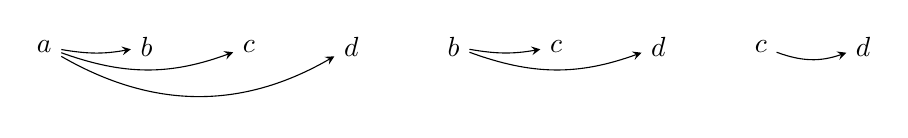
\begin{tikzpicture}[>=stealth, scale=1.3]
\node(A1) at (0,0){$a$};
\node(A2) at (1,0){$b$};
\node(A3) at (2,0){$c$};
\node(A4) at (3,0){$d$};
\node(B1) at (4,0){$b$};
\node(B2) at (5,0){$c$};
\node(B3) at (6,0){$d$};
\node(C1) at (7,0){$c$};
\node(C2) at (8,0){$d$};

\draw[->](A1) to [bend left=-10](A2);
\draw[->](A1) to [bend left=-20](A3);
\draw[->](A1) to [bend left=-30](A4);
\draw[->](B1) to [bend left=-10](B2);
\draw[->](B1) to [bend left=-20](B3);
\draw[->](C1) to [bend left=-20](C2);
\end{tikzpicture}
    \caption{}
\end{figure}

如图7.7所表示的，先写字母$a$依次与$b,c,d$的组合，再写字母$b$依次与$c,d$的组合，再写字母$c$与$d$的组合，由此可以写出$a,b,c,d$这4个元素中每次取出2个元素的所有组合：
\[ab,\quad ac,\quad ad,\quad bc,\quad bd,\quad cd\]
\end{solution}

\section{组合数公式}

从$n$个不同元素中取出$m\; (m\le n)$ 个元素的所有组合的个数，叫做从$n$个不同元素中取出$m$个元素的\textbf{组合数}，用符号$\comb{n}{m}$ 表示\footnote{C是英文Combination（组合）的第一个字母。}。

例如，从5个不同元素中取出2个元素的组合数表示成$\comb{5}{2}$; 从10个不同元素中取出7个元素的组合数表示成$\comb{10}{7}$.

为了寻求组合数的计算公式，我们先来比较一下已学过的排列和现在研究的组合这两个概念的异同点及其联系。

显然，两个定义所叙述的都是从$n$个不同元素中任取$m$个元素，但组合是取出来后放在一起成为一组就行了，而排列还要把这$m$个元素按不同的顺序排出所有的情况。所以排列要比组合多一步，即要按不同的顺序把$m$个元素排出各种情况。

例如，从4个不同元素$a,b,c,d$取出2个元素的排列与组合的关系如下表所示：
\begin{center}
\begin{tikzpicture}[>=stealth, scale=.7]
\node at(0,4){组合};
\node at (5,4){排列};
\node (A1) at (0,3) {$a,\; b$};
\node (B1) at (5,3) {$ab,\; ba$};
\node (A2) at (0,2) {$a,\; c$};
\node (B2) at (5,2) {$ac,\; ca$};
\node (A3) at (0,1) {$a,\; d$};
\node (B3) at (5,1) {$ad,\; da$};
\node(A4) at (0,0) {$b,\; c$};
\node (B4) at (5,0) {$bc,\; cb$};
\node (A5) at (0,-1) {$b,\; d$};
\node (B5) at (5,-1) {$bd,\; db$};
\node (A6) at (0,-2) {$c,\; d$};
\node (B6) at (5,-2) {$cd,\; dc$};

\foreach \x in {3,2,1,...,-2}
{
    \draw(-1,\x-.4) rectangle (1,\x+.4);
    \draw(3.5,\x-.4) rectangle (6.5,\x+.4);
    \draw[->](1,\x)--(3.5,\x);
}


\end{tikzpicture}
\end{center}

在找到了它们之间的区别与联系后，对于排列数$\perm{n}{m}$, 我们又可有新的处理方法。

第一步，先从$n$个元素中选取$m$个元素放在一起（就是组成一组），显然这一步骤完成的方法数就是组合数$\comb{n}{m}$;

第二步，再求出$m$个元素的全排列数$\perm{n}{m}$.

根据排列数的定义和乘法原理可得：
\[
\perm{n}{m}=\comb{n}{m}\cdot \perm{m}{m}.\]

这个关系不仅揭示了排列数与组合数的联系，而且给出了组合数的计算公式。因此有
\[\comb{n}{m}=\frac{\perm{n}{m}}{\perm{m}{m}}=\frac{n(n-1)(n-2)\cdots(n-m+1)}{m!}\]
这里$n, m\in \N$，并且$m\le  n$. 这个公式叫做\textbf{组合数公式}。

因为
\[\perm{n}{m}=\frac{n!}{(n-m)!}\]

所以，上面的组合数公式还可以写成
\[\comb{n}{m}=\frac{n!}{m!(n-m)!}\]
这也是组合数的一个常用公式。

\begin{example}
    计算下列各题：
\begin{multicols}{3}
\begin{enumerate}[(1)]
    \item $\comb{9}{3}$;
    \item $\comb{9}{4}$;
    \item $\comb{8}{5}$.
\end{enumerate}    
\end{multicols}
\end{example}


\begin{solution}
\begin{enumerate}[(1)]
    \item $\comb{9}{3}=\frac{9\x  8\x  7}{3\x  2\x  1}=84$;
    \item $\comb{9}{4}=\frac{9\x  8\x  7\x  6}{4\x  3\x  2\x  1}=126$;
    \item $\comb{8}{5}=\frac{8\x  7\x  6\x  5\x  4}{5\x  4\x  3\x  2\x  1}=56$.
\end{enumerate}
\end{solution}

\begin{example}
    求证
\begin{multicols}{2}
\begin{enumerate}[(1)]
    \item $\comb{n}{m}=\frac{m+1}{n-m}\comb{n}{m+1}$;
    \item $\comb{n}{m}=\frac{n}{m}\comb{n-1}{m-1}$.
\end{enumerate}
\end{multicols}
\end{example}

\begin{proof}
\begin{enumerate}[(1)]
    \item $\because\quad \comb{n}{m}=\frac{n!}{m!(n-m)!}$

\[\begin{split}
\frac{m+1}{n-m}\comb{n}{m+1}&=\frac{m+1}{n-m}\cdot \frac{n!}{(m+1)!(n-m-1)!}\\
& =\frac{m+1}{(m+1)!}\cdot \frac{n!}{(n-m)(n-m-1)!}\\
&=\frac{n!}{m!(n-m)!}
\end{split}\]

$\therefore\quad \comb{n}{m}=\frac{m+ 1}{n-m}\comb{n}{m+1}$.

    \item $\because\quad \comb{n}{m}=\frac{n!}{m!(n-m)!}$,

\[\frac{n}{m}\comb{n-1}{m-1}=\frac{n}{m}\cdot \frac{(n-1)!}{(m-1)!(n-m)!}=\frac{n!}{m!(n-m)!}.\]

$\therefore\quad \comb{n}{m}=\frac{n}{m}\comb{n-1}{m-1}$.
\end{enumerate}
\end{proof}


\begin{ex}
\begin{enumerate}
    \item $A,B,C,D$四个球队举行单循环比赛：
\begin{enumerate}[(1)]
    \item 列出所有比赛的双方；
    \item 列出所有冠亚军的可能情况。
\end{enumerate}
\item 某校举行篮球单循环赛，有6个队参加，共需举行多少场比赛？
\item 写出从五个元素$a,b,c,d,e$中任取三个元素的所有组合。
\item 计算：
\begin{multicols}{2}
\begin{enumerate}[(1)]
    \item $\comb{5}{2}$;
    \item $\comb{6}{3}$;
    \item $\comb{8}{8}$;
    \item $\comb{7}{3}-\comb{6}{2}$;
\item $\comb{5}{1}+\comb{5}{2}+\comb{5}{3}+\comb{5}{4}+\comb{5}{5}$.
\end{enumerate}
\end{multicols}
\item 从数2310的质因数中，每次取出两个相乘，可以得到多少个不相等的积？
\end{enumerate}
 \end{ex}   

